\section{Additional comments}
Here it follows a list of consideration and comments, that we would like to point out:
\begin{itemize}
\item The implementation and testing document, in our opinion, misses some points. 
In particular, a discussion on how the frameworks adopted match, in some sense, the requirements and the goal of the project 
is not present at all: what is possible to find is only a list of advantages and disadvantages of the framework, and most of them are not
related to the system developed, but very general
\item Motivations regarding the choice of implemented features of automated SOS is not present at all
\item In the section regarding the test, it is said that "tests were done by hand"
This choice has not been motivated and, of course, it presents obvious disadvantages: it is necessary to repeat all the tests as soon as
an update or fix is released
\item Most of the code that we looked at, in particular the backend, misses most of the documentation. For very few methods, some sort
of comments is present
\item Even if is present a sort of domain assumptions regarding security (i.e. D2 TrackMe addresses data protection and integrity against
possible attacks), it is not clear what this concerns. Therefore, since we considered important, as users, to don't access APIs that
concerns other users, we have tested also this possibility. \\
One should also note that password are saved in clear.
TODO FIX THIS IS NOT TEST ARE PERFORMED AT THE END
\item It is not clear why, for accepting a request, it is requested to use also the SSN: the token should be the only thing relevant, from a
API design point of view
\item The code of aos.js misses, for some reason, all sort of indentation
\item No information regarding the coverage of the test is present in the documentation provided. 
Any kind of report is missing, in this sense: to us, this seems to be useful information
\item While searching for individual data, if a wrong SSN is inserted first, and then 
a correct one, the error message does not disappear. 

\begin{figure}[H]
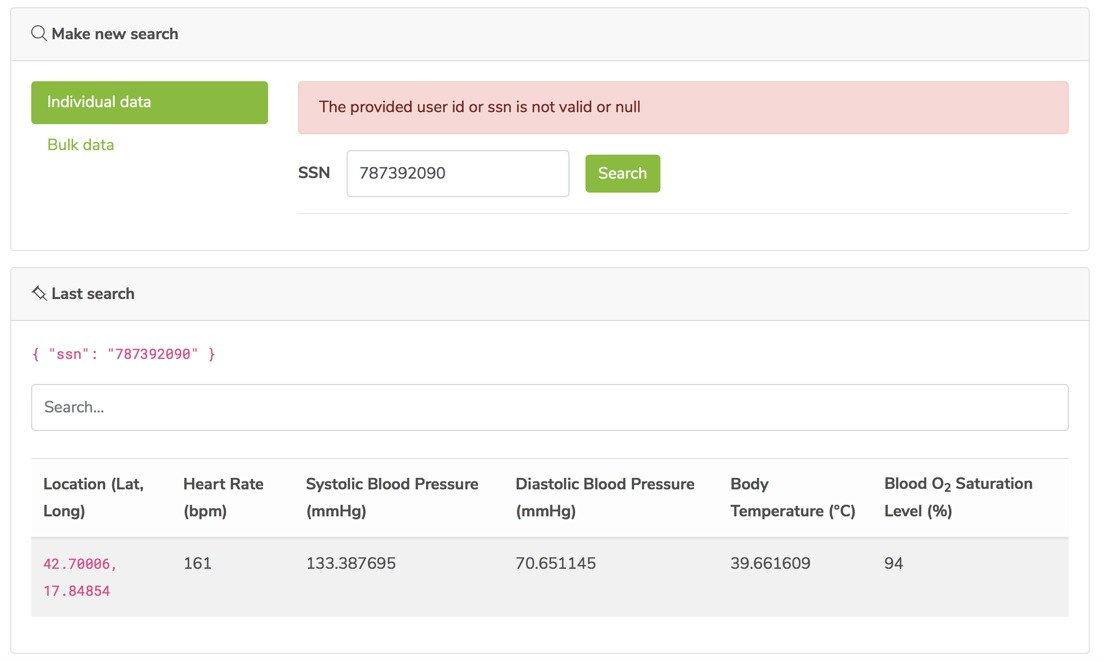
\includegraphics[width=\linewidth]{images/bug1.png}
\caption{ UI bug }
\label{fig:bug1}
\end{figure}

Other mini bugs like this are present. However, they are not important since the 
UI is not considered to be the main purpose of the project. \\
This one has been reported as an example, for the sake of completeness.
\end{itemize}